\title{GPG in Linux}
\author{Chari Karipidis\\
		2TinG\\}
\date{\today}

\documentclass[12pt]{article}

\usepackage{graphicx}
\usepackage{fancyhdr}
\pagestyle{fancy}
\lhead{Chari Karipidis}
\chead{}
\rhead{2TinG}
\lfoot{}
\cfoot{\thepage}
\rfoot{}
\renewcommand{\headrulewidth}{0.4pt}
\renewcommand{\footrulewidth}{0.4pt}

\begin{document}
\maketitle

\newpage
\tableofcontents

\newpage
\section{Introductie}
In dit document wordt het gebruik van GPG(GnuPG) nader verklaard.

\paragraph{Benadering}
De geschiedenis, werking en uitvoer wordt utgewerkt in Sectie~\ref{GPG} GPG.\\
Sectie~\ref{Belangrijke woorden} Belangrijke woorden, geeft een overzicht van belangrijke woorden in het document.

\newpage
\section{GPG}\label{GPG}
\subsection{Geschiedenis}
Er is altijd wel een probleem met boodschappen verzenden en ontvangen, zonder dat men deze kunnen onderscheppen en lezen. Hier zijn handige uitvingen voor ontworpen, die helpen bij dit probleem.

\paragraph{Scytale}
In de tijd van de romeinen had men een manier nodig om berichten te versturen naar geallieerde troepen. Verzender en ontvanger waren in het bezit van een 'Scytale' van ieder dezelfde grootte. Dit voorwerp was een soort van cilinder. Hier werd een riem over gewikkeld en een boodschap op geschreven.\\
Bij het verwijderen van de riem, was deze tekst onleesbaar zonder behulp van de Scytale. De letters waren namelijk door mekaar. Bij ontvangts van de riem bij de troepen, wikkelde ze de riem over de Scytale die zij bezitte en was het zo mogelijk, de boodschap te lezen.\\
Dit was een soort van encryptie. Ervoor zorgen dat een onderschepper, de boodschap niet kan lezen.

\paragraph{Caesar methode}
Een andere encryptie-methode was de Caesar methode.\\
Deze bestond uit een zin hervormen m.b.v. het alphabet. Dit klinkt natuurlijk zeer logisch.
Het alphabet wordt namelijk gebruikt om zinnen te schrijven.\\
Maar na het schrijven van de nodige boodschap, wordt er een 'sleutel' gekozen. Deze sleutel is afgesproken cijfer tussen 1 en 26, tussen beide partijen.\\
Belangrijk is dat de cijfers overeenkomen met een letter uit het alphabet. Als het gekozen cijfer, 6 is. Wordt het alphabet 6 maal naar links verschoven. A wordt dan F en B wordt dan G, enz...\\
De ontvanger krijgt dan een wirwar van letters en kan deze ontcijferen door het alphabet terug te vormen foor het 6 maal naar rechts te verschuiven.\\


Tegenwoordig worden loopjongens niet meer gebruikt. Men is mee geevolueerd naar de toekomst.\\
Technology is nu de heerser over het verzenden van boodschappen.
Mailen, accounts aanmaken, bestanden opslaan, enz... Gebeurt iedere dag. Dit moet dan ook beveiligd worden.\\
Een manier voor encryptie is GPG.

\newpage
\subsection{Wat is GPG?}
GPG of GnuPG staat voor; Gnu Privacy Guard. Zoals de naam al voorstelt, is het om de privacy van gebruikers te beschermen. Dit doormiddel van encryptie van boodschappen die verzonden moeten worden zoals mails, data encrypteren, 'sleutelhangers', enz... \\
GnuPG is een commando voor de terminal, maar er zijn dergelijke frontend programma's om deze in een gui te kunnen gebruiken. Te zien in Subsectie~\ref{GUI}

\subsection{Frontend GPG programma's}\label{GUI}
\begin{center}
\begin{tabular}{r|l}
Cryptophane	&	Een applicatie voor Windows.\\
Gajim		&	Een Jabber client voor GNOME.\\
GnuPG Shell	&	Een cross-platform, grafische Frontend voor GnuPG.\\
GPA			&	De standaard Frontend voor GPG.\\
KGpg		&	GnuPG voor KDE.\\
Seahorse	&	GnuPG voor GNOME.\\
Wija		&	Een cross-platform jabber client (MacOsX, Linux, Windows).\\
\end{tabular}
\end{center}

\paragraph{Cryptophane}
Deze wordt gebruikt om te encrypteren, decrypteren, handtekenen, beheer van sleutelhanger en een command-line interface voor GnuPG.\\
\begin{center}
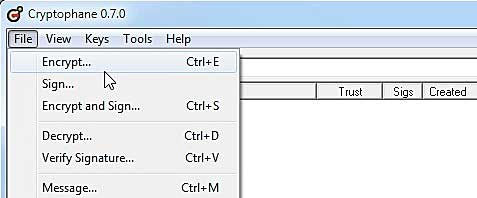
\includegraphics[scale=0.6]{Pictures/cryptophane}
\end{center}

\paragraph{Gajim}
Gajim is een Jabber-client. Een Jabber-client is een messaging applicatie.
Omdat Gajim werkt met GnuPG, zullen de berichten die verzonden worden met Gajim, Geincrypteerd worden.
\begin{center}
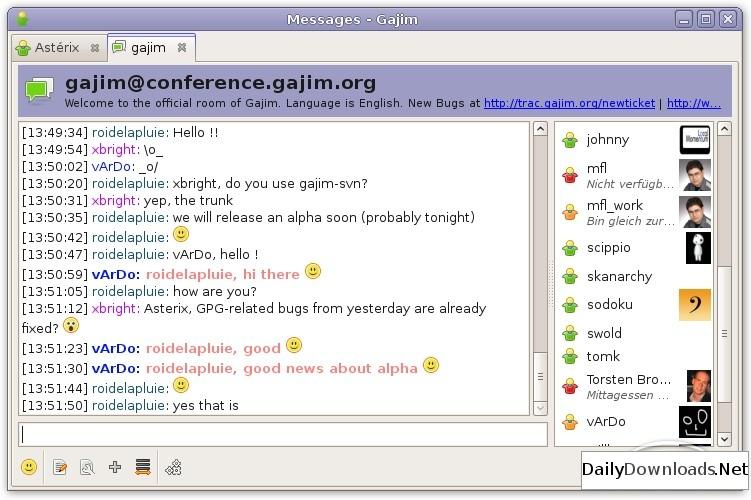
\includegraphics[scale=0.4]{Pictures/gajim}
\end{center}

\paragraph{GPGshell}
Een grafische frontend voor iedere platform. Met deze GUI is het mogelijk sleutels bij te houden en te encrypteren. 
\begin{center}
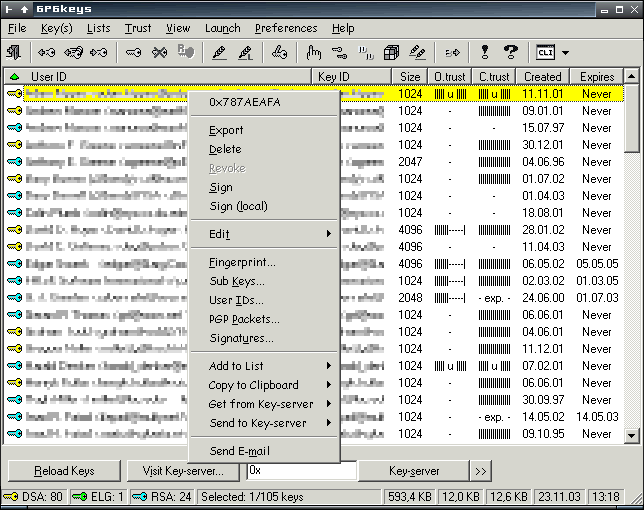
\includegraphics[scale=0.5]{Pictures/gpgshell}
\end{center}

\paragraph{GPA}
GPA probeert de standaard frontend te zijn voor GPG. $www.gnupg.org$ Host GPA.
\begin{center}
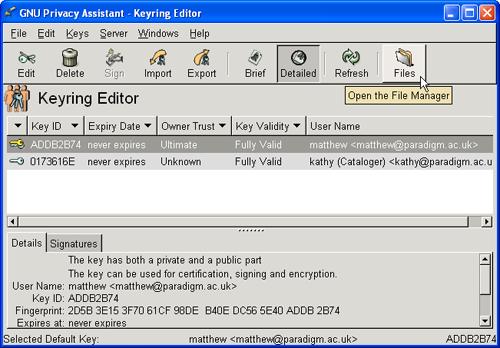
\includegraphics[scale=0.6]{Pictures/GPA}
\end{center}

\paragraph{KGpg}
Met KGpg kan je bestanden en mails encrypteren en dycrepteren om je informatie veilig te houden.
Het is een gratis en open-source frontend.
\begin{center}
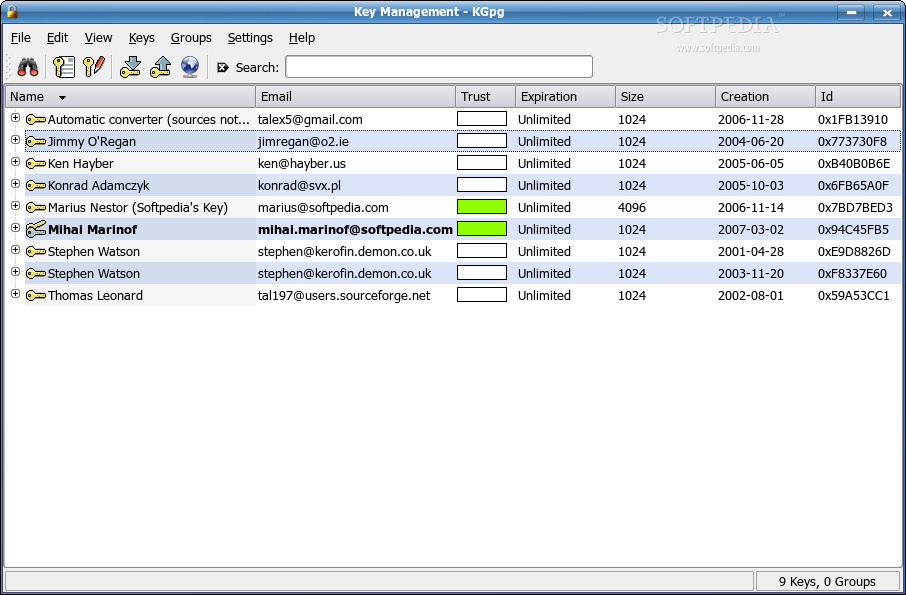
\includegraphics[scale=0.3]{Pictures/kgpg}
\end{center}

\paragraph{Seahorse}
Seahorse is een GUI voor GNOME. Het is ook geintegreerd in Nautilus, gedit en andere applicaties voor encryptie uit te voeren.
Je kan met Seahorse; PGP en SSH sleutels maken en beheren, publiceren en terughalen van sleutels op de servers, een passphrase cachen, sleutelhanger backuppen, enz...
\begin{center}
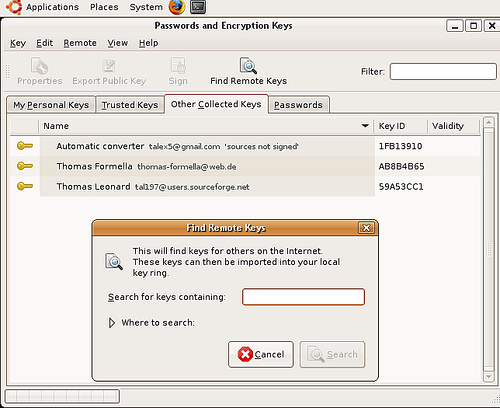
\includegraphics[scale=0.5]{Pictures/Seahorse}
\end{center}

\paragraph{Wija}
Een Jabber-client zoals Gajim, maar geschreven in java en beschibaar voor ieder platform.
Het heeft een ingebouwde sleutelhanger beheersysteem. Het kan ook zeer gemakkelijk boodschappen encrypteren en dycrepteren voor gewone gesprekken of multi-user gesprekken.
Het is ook mogelijk de boodschappen te handtekenen.
\begin{center}
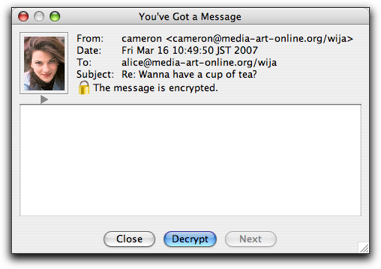
\includegraphics[scale=0.7]{Pictures/wija}
\end{center}

\newpage
\section{Belangrijke woorden}\label{Belangrijke woorden}
\begin{tabular}{r|l}
Jabber-client		&	\\
Cross-platform		&	\\
Multi-user			&	\\
\end{tabular}

\newpage
\section{Referenties}\label{Referenties}
$http://www.jumaros.de/rsoft/index.html$ \\
$http://www.gnupg.org/related_software/frontends.en.html$ \\
$http://www.google.be$
$http://utils.kde.org/projects/kgpg/$
$http://projects.gnome.org/seahorse/$

\bibliographystyle{abbrv}
\bibliography{myID}

\end{document}
